\documentclass[a4paper,12pt]{article}
\usepackage{graphicx}
\usepackage{geometry}
\usepackage{float}
\title{Best-of-n}
\author{Zixuan Liu\thanks{University of Bristol}}
\geometry{left = 2.5cm, right = 2.5cm,top = 2.5cm}
\usepackage{pstricks}
\usepackage{listings}
\usepackage{color}
%\usepackage{gnuplot-lua-tikz}
\usepackage{tikz}

\usepackage{pgf}
\usepackage[utf8]{inputenc}
\usetikzlibrary{arrows,automata}
\usetikzlibrary{positioning}


\tikzset{
	state/.style={
		rectangle,
		rounded corners,
		draw=black, very thick,
		inner sep=2pt,
		text centered,
	},
}
\tikzset{
	on/.style={
		circle,
		draw=red, very thick,
		inner sep=2pt,
		fill=red!25,
	},
}


\tikzset{
	off/.style={
		circle,
		draw=blue, very thick,
		inner sep=2pt,
		text centered,
	},
}



\tikzset{
	neuron/.style={
		rectangle,
		rounded corners,
		draw=black, very thick,
		inner sep=2pt,
		text centered,
	},
}



\tikzset{
	area/.style={
		rectangle,
		draw=black, very thick,
		inner sep=2pt,
		text centered,
	},
}


\tikzset{
	gc/.style={
		rectangle,
		rounded corners,
		draw=red, very thick,
		inner sep=2pt,
		text centered,
	},
}


\tikzset{
	inh/.style={
		rectangle,
		rounded corners,
		draw=blue, very thick,
		inner sep=2pt,
		text centered,
	},
}



\tikzset{
	io/.style={
		rectangle,
		draw=green, very thick,
		inner sep=2pt,
		text centered,
	},
}
\begin{document}
	\maketitle
	%\section*{Figures in section~1 to~4 similarity was caled by 1st version(with some problem)} 
	\section{n = 10 and 3000 iteration with 200 agents}\label{SRRI}
	Grid : Q = {'H0':1,'H1': 12, 'H2': 7, 'H3': 8, 'H4': 6,'H5': 3,'H6': 2,'H7': 4,'H8':5,'H9':1}
	\graphicspath{{figs/}}
	Time used: 270~${s}$
	\begin{figure}[H]
		\centering
		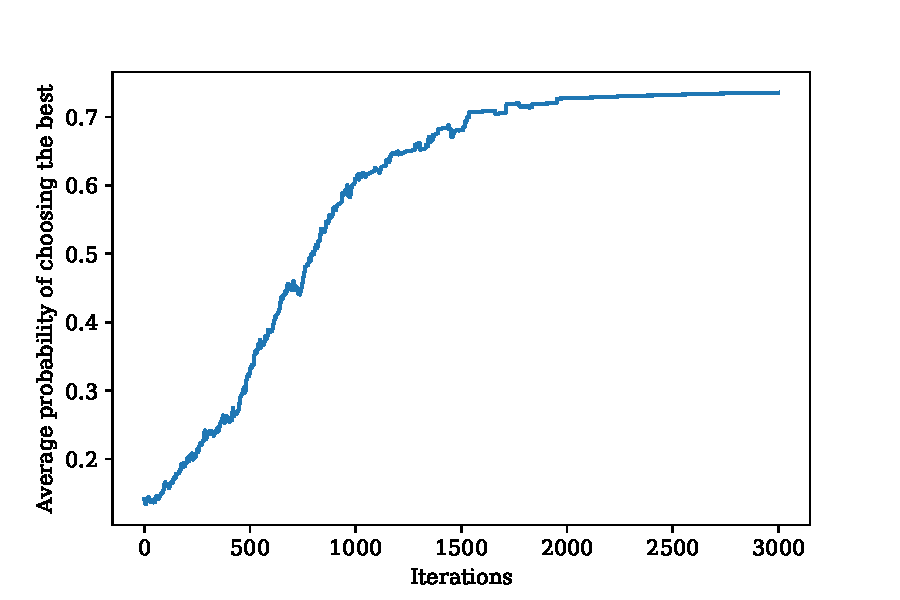
\includegraphics[width=0.9\textwidth]{Average_pbest200_3000}
		\caption{Probability for choosing the best against iteration time, average of 100 time run}\label{Average_pbest200_3000}
	\end{figure}
%
	\begin{figure}[H]
		\centering
		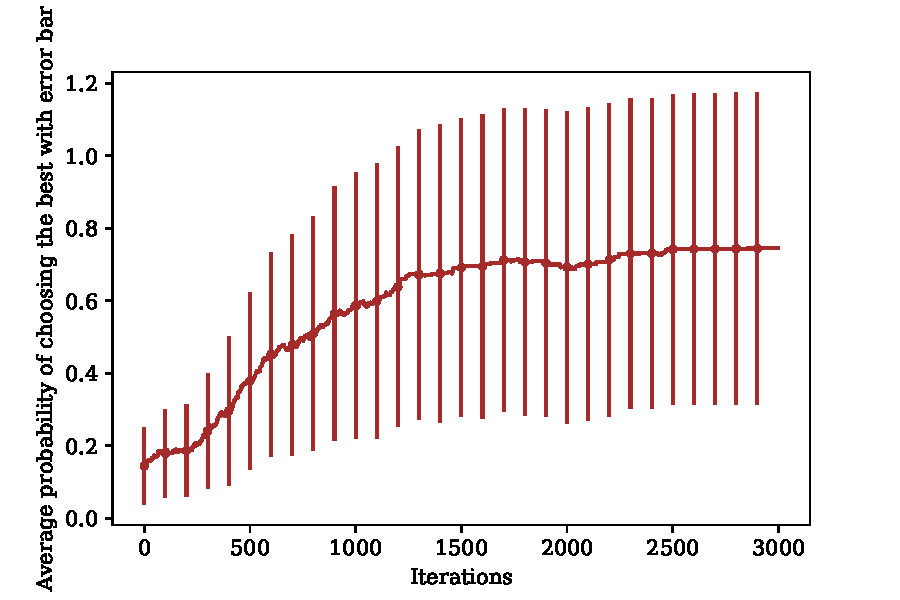
\includegraphics[width=0.9\textwidth]{Average_pbest_errbar200_3000}
		\caption{Probability for choosing the best against iteration time, average of 100 time run, with error bar}\label{Average_pbest_errbar200_3000}
	\end{figure}
	%
	\begin{figure}[H]
		\centering
		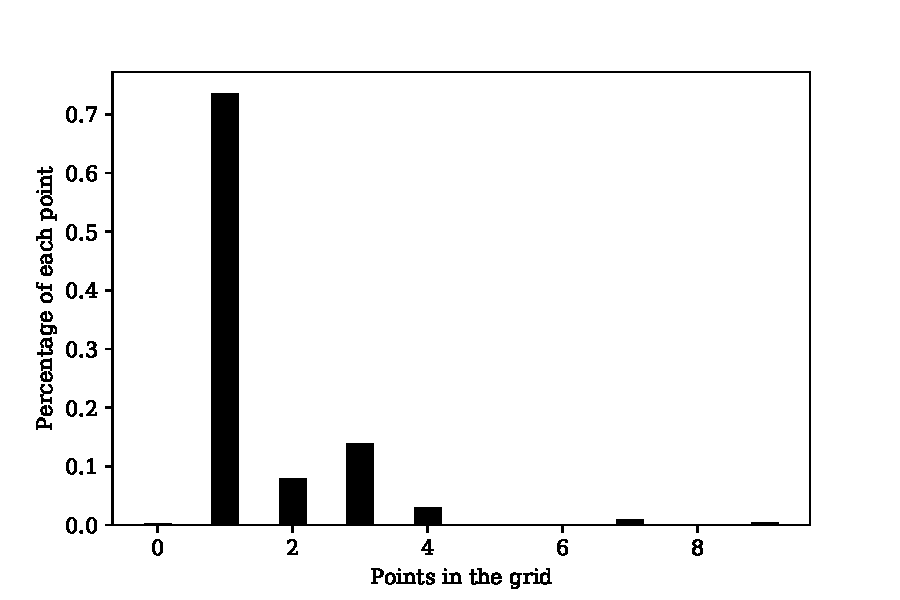
\includegraphics[width=0.9\textwidth]{average_percentage200_3000}
		\caption{percentage of converging to the best, average of 100 time run, Histogram}\label{average_percentage200_3000}
	\end{figure}
	\begin{figure}[H]
		\centering
		\includegraphics[width=0.9\textwidth]{average_percentage200_3000_2}
		\caption{average percentage average of choosing to the best, average of 100 time run, circle}\label{average_percentage200_3000_2}
	\end{figure}
	\begin{figure}[H]
	\centering
	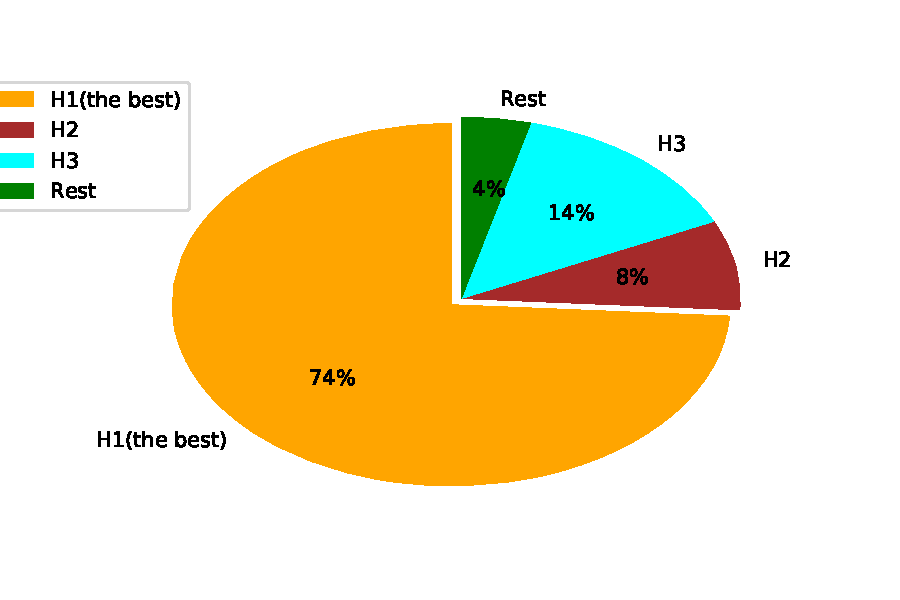
\includegraphics[width=0.9\textwidth]{average_percentage200_3000_3}
	\caption{percentage of converging to the best, average of 100 time run, pie}\label{average_percentage200_3000_3}
	\end{figure}

	\begin{figure}[H]
		\centering
		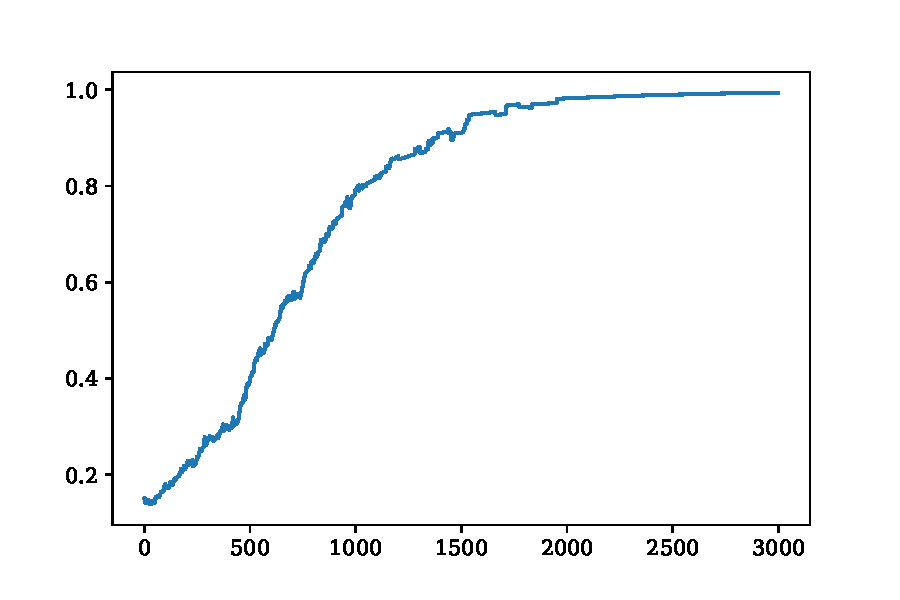
\includegraphics[width=0.9\textwidth]{correct_pbest200_3000}
		\caption{Probability for choosing the best against iteration time, average of 100 time run, only when converge to the best of n(H1)}\label{correct_pbest200_3000}
	\end{figure}
	\begin{figure}[H]
		\centering
		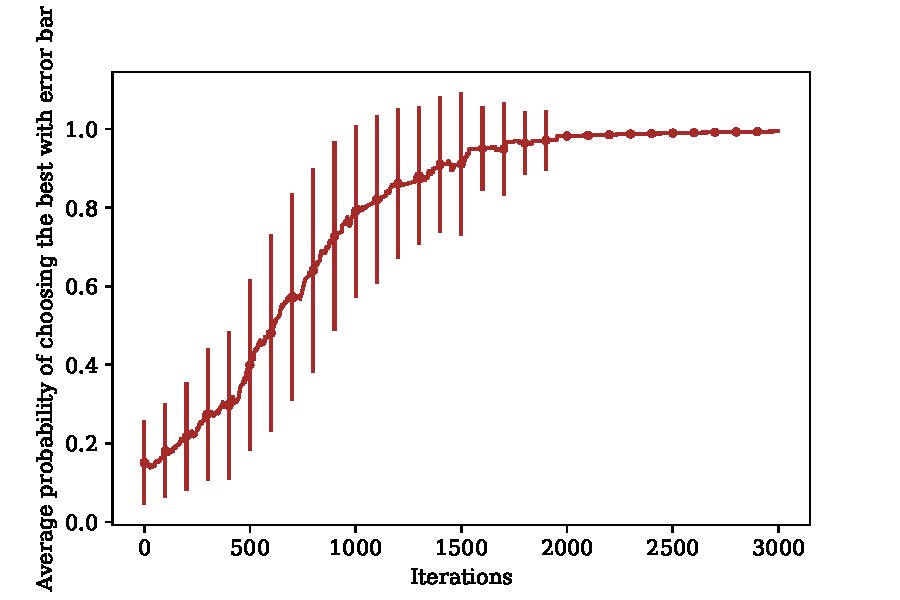
\includegraphics[width=0.9\textwidth]{correct_pbest_errbar200_3000}
		\caption{Probability for choosing the best against iteration time, average of 100 time run, only when converge to the best of n(H1), with error bar}\label{correct_pbest_errbar200_3000}
	\end{figure}
%
	\begin{figure}[H]
	\centering
	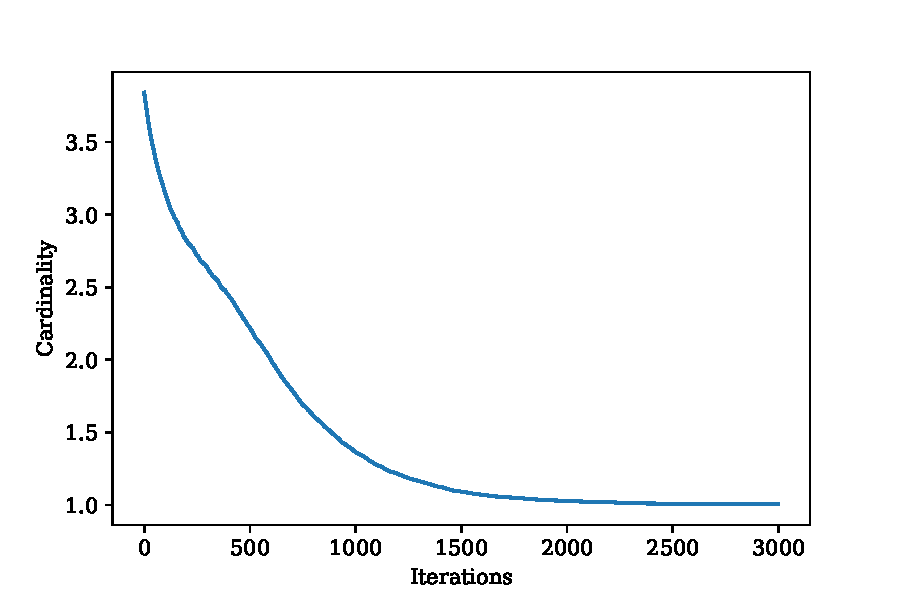
\includegraphics[width=0.9\textwidth]{card200_3000}
	\caption{Cardinality against iteration time, average of 100 time run}\label{card200_3000}
	\end{figure}
	\begin{figure}[H]
		\centering
		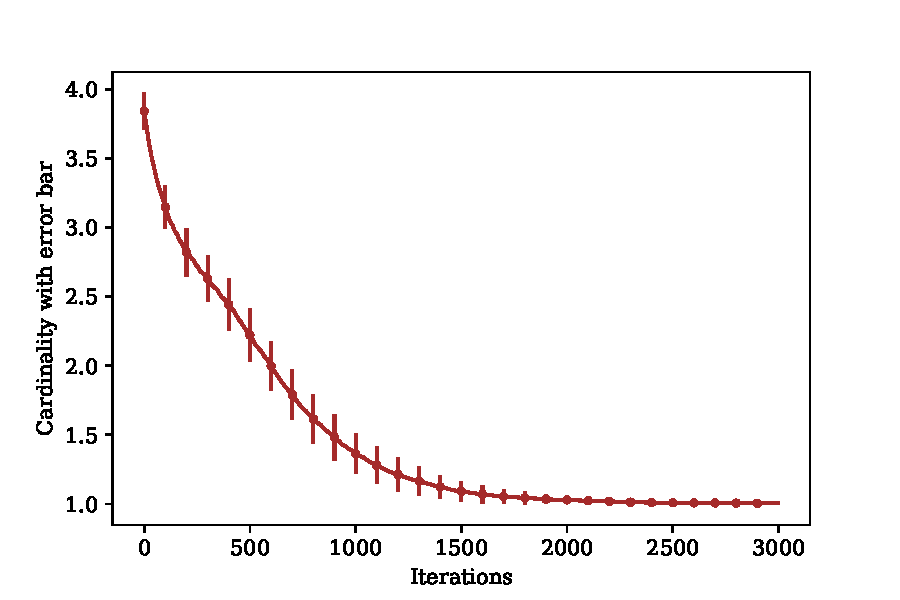
\includegraphics[width=0.9\textwidth]{card_errbar200_3000}
		\caption{Cardinality against iteration time, average of 100 time run, with error bar}\label{card_errbar200_3000}
	\end{figure}
\section{n = 10 and 3000 iteration with 200 agents which are picked based on squared rank}\label{sqrank}
\subsection{100 times experiments}
	Grid : Q = \{'H0':1,'H1': 12, 'H2': 7, 'H3': 8, 'H4': 6,'H5': 3,'H6': 2,'H7': 4,'H8':5,'H9':1\}
	The probability was determined by the square of rank of points' qualities.
	\graphicspath{{figsNorm1/}}
	Time used: 364~${s}$
	\begin{figure}[H]
		\centering
		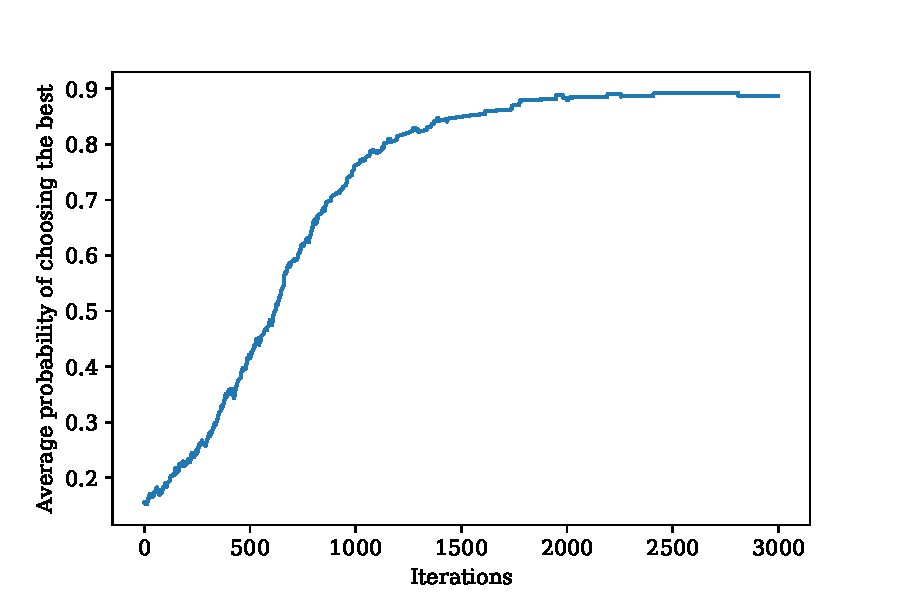
\includegraphics[width=0.9\textwidth]{Average_pbestnorm1_200_3000_100}
		\caption{Probability for choosing the best against iteration time, average of 100 time run}\label{Average_pbestnorm1_200_3000_100}
	\end{figure}
	%
	\begin{figure}[H]
		\centering
		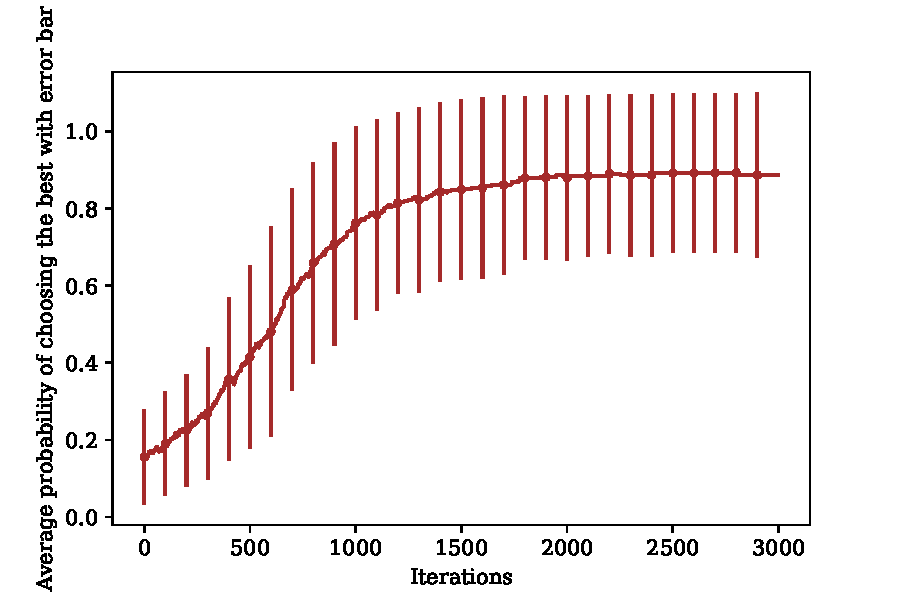
\includegraphics[width=0.9\textwidth]{Average_pbest_errbarnorm1_200_3000_100}
		\caption{Probability for choosing the best against iteration time, average of 100 time run, with error bar}\label{Average_pbest_errbarnorm1_200_3000_100}
	\end{figure}
	%
	\begin{figure}[H]
		\centering
		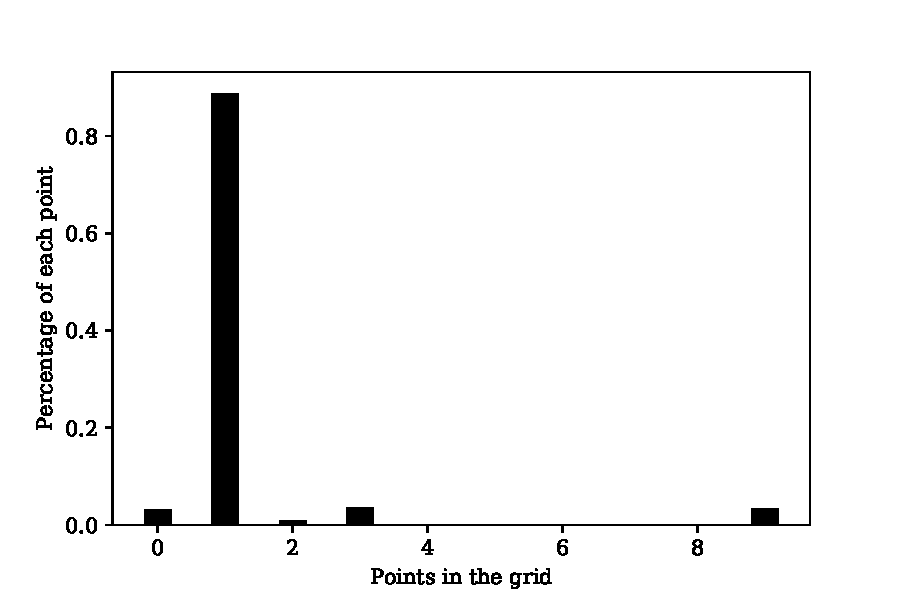
\includegraphics[width=0.9\textwidth]{average_percentagenorm1_200_3000_100}
		\caption{percentage of converging to the best, average of 100 time run, Histogram}\label{average_percentagenorm1_200_3000_100}
	\end{figure}
	\begin{figure}[H]
		\centering
		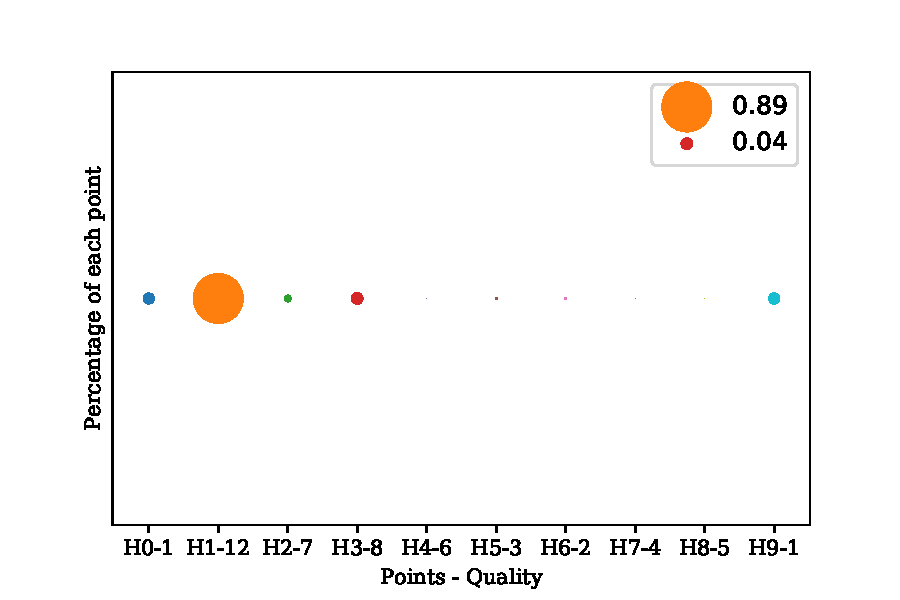
\includegraphics[width=0.9\textwidth]{Average_percentagenorm1_200_3000_100_2}
		\caption{average percentage average of choosing to the best, average of 100 time run, circle}\label{Average_percentagenorm1_200_3000_100_2}
	\end{figure}
	\begin{figure}[H]
		\centering
		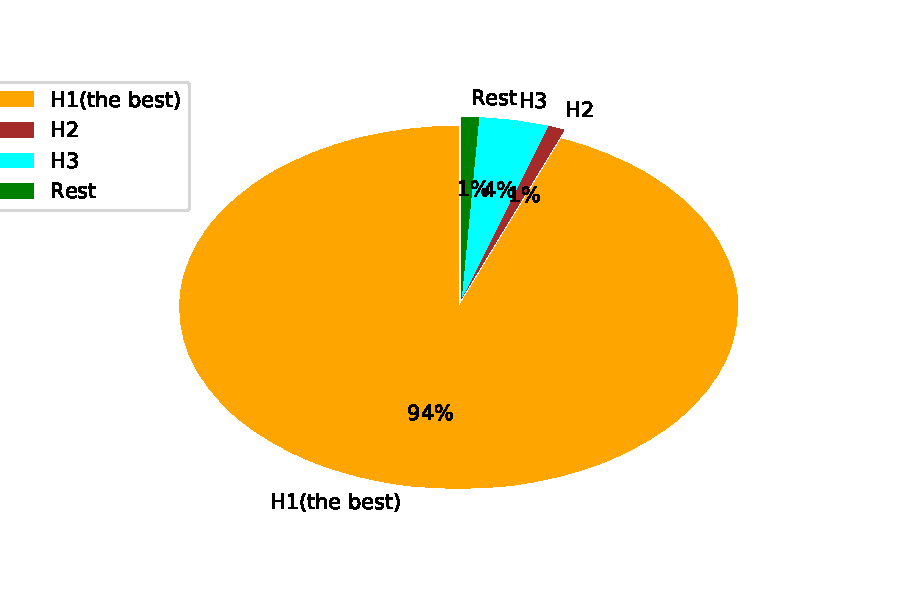
\includegraphics[width=0.9\textwidth]{average_percentagenorm1_200_3000_100_3}
		\caption{percentage of converging to the best, average of 100 time run, pie}\label{average_percentagenorm1_200_3000_100_3}
	\end{figure}
	
	\begin{figure}[H]
		\centering
		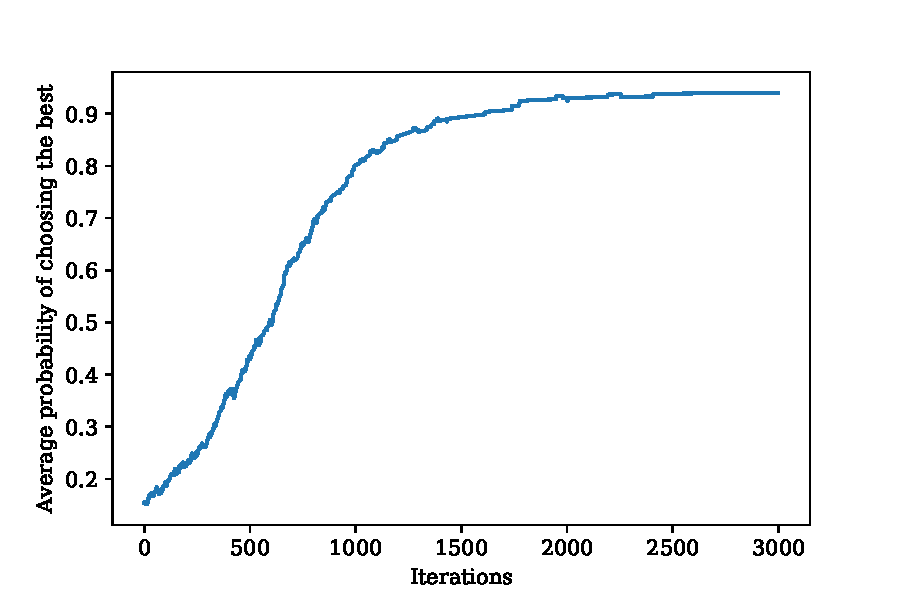
\includegraphics[width=0.9\textwidth]{correct_pbestnorm1_200_3000_100}
		\caption{Probability for choosing the best against iteration time, average of 100 time run, only when converge to the best of n(H1)}\label{correct_pbestnorm1_200_3000_100}
	\end{figure}
	\begin{figure}[H]
		\centering
		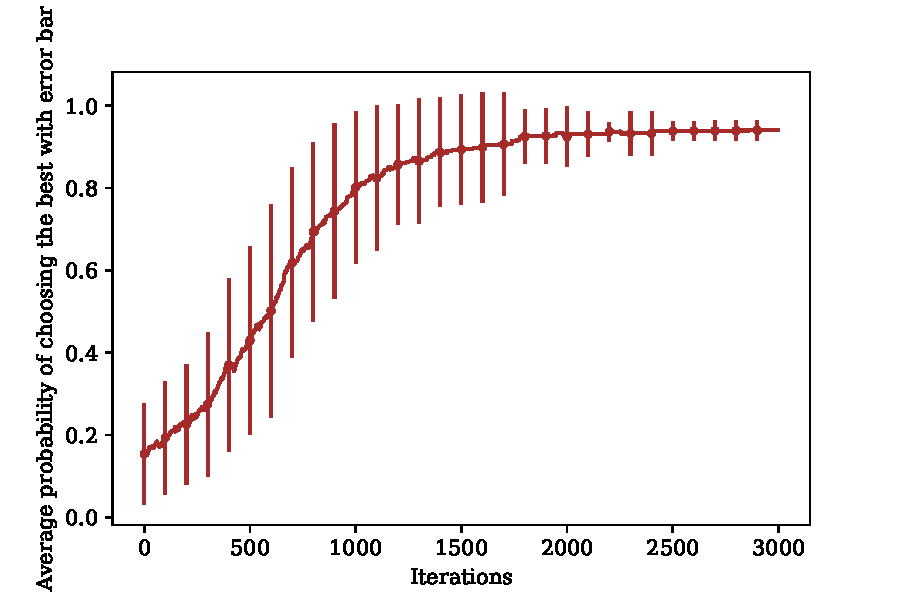
\includegraphics[width=0.9\textwidth]{correct_pbest_errbarnorm1_200_3000_100}
		\caption{Probability for choosing the best against iteration time, average of 100 time run, only when converge to the best of n(H1), with error bar}\label{correct_pbest_errbarnorm1_200_3000_100}
	\end{figure}
	%
	\begin{figure}[H]
		\centering
		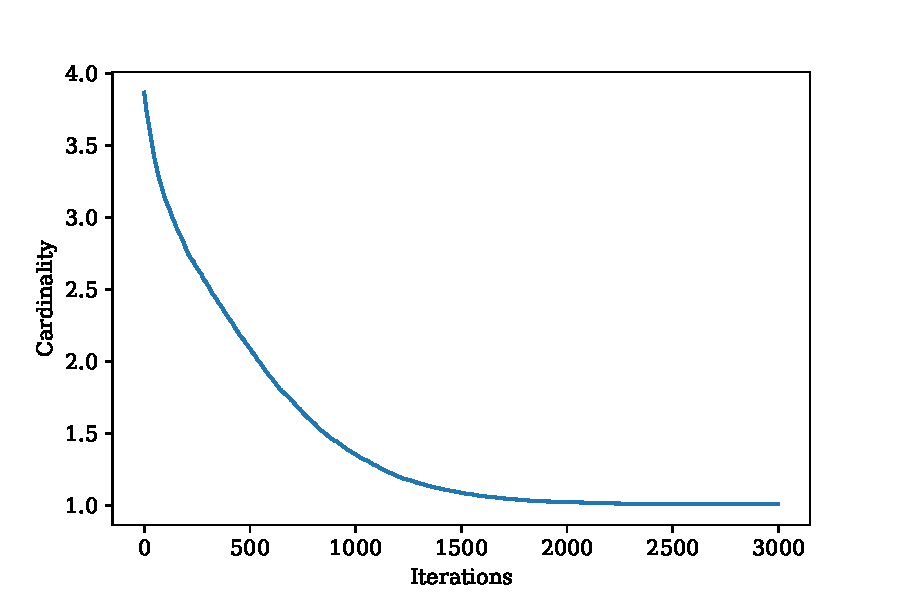
\includegraphics[width=0.9\textwidth]{cardnorm1_200_3000_100}
		\caption{Cardinality against iteration time, average of 100 time run}\label{cardnorm1_200_3000_100}
	\end{figure}
	\begin{figure}[H]
		\centering
		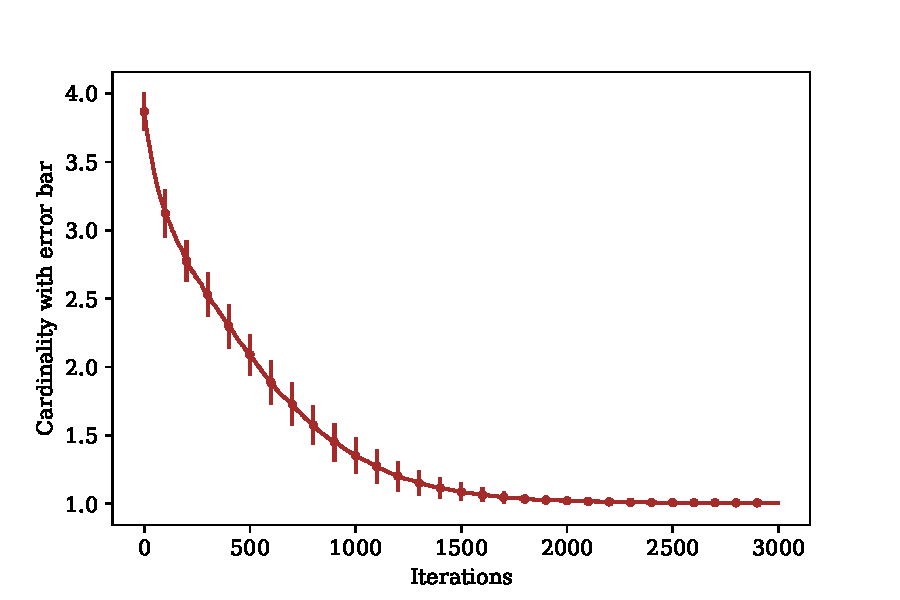
\includegraphics[width=0.9\textwidth]{card_errbarnorm1_200_3000_100}
		\caption{Cardinality against iteration time, average of 100 time run, with error bar}\label{card_errbarnorm1_200_3000_100}
	\end{figure}
\subsection{500 times experiments}
	%\graphicspath{{figsNorm1/}}
	Time used: 1813.9~${s}$
	\begin{figure}[H]
		\centering
		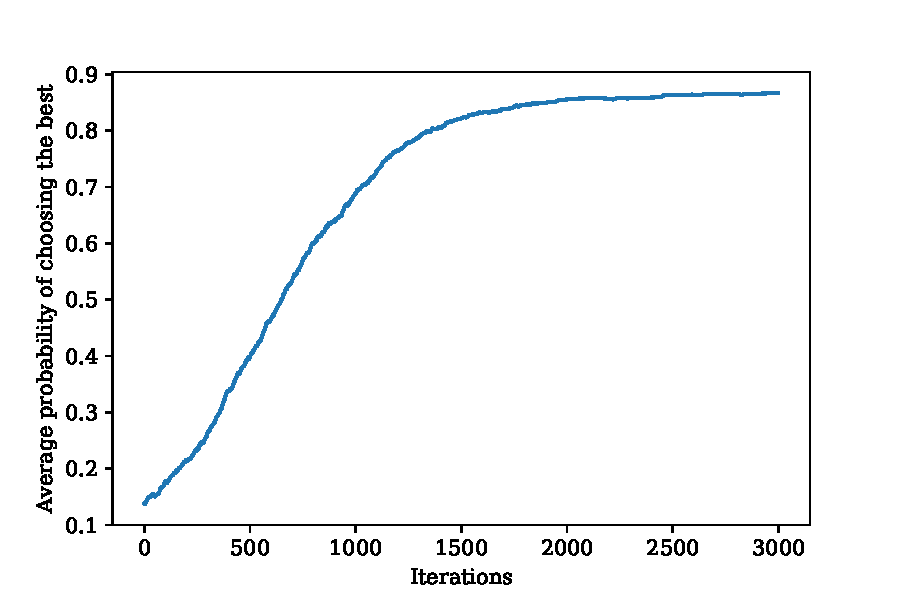
\includegraphics[width=0.9\textwidth]{Average_pbestnorm1_200_3000_500}
		\caption{Probability for choosing the best against iteration time, average of 500 time run}\label{Average_pbestnorm1_200_3000_500}
	\end{figure}
	%
	\begin{figure}[H]
		\centering
		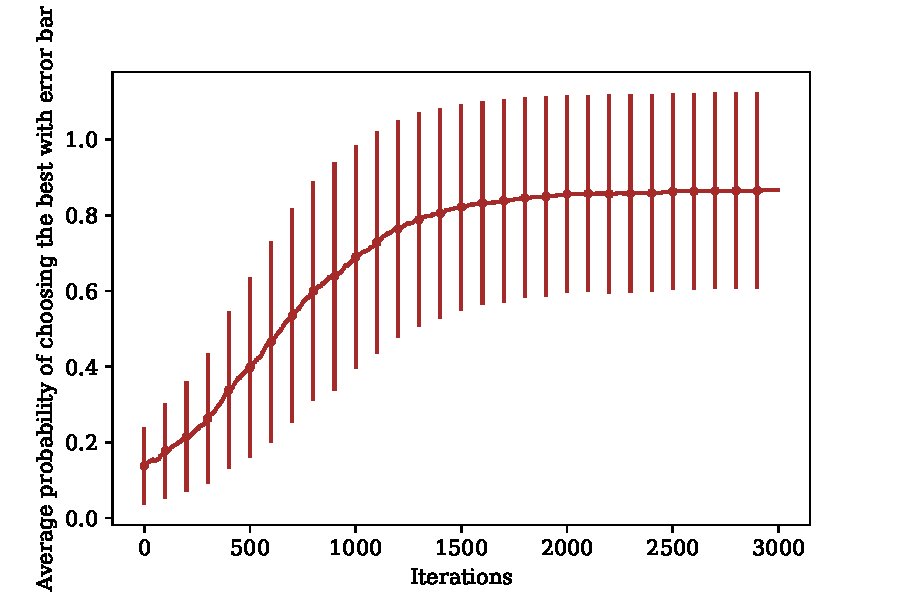
\includegraphics[width=0.9\textwidth]{Average_pbest_errbarnorm1_200_3000_500}
		\caption{Probability for choosing the best against iteration time, average of 500 time run, with error bar}\label{Average_pbest_errbarnorm1_200_3000_500}
	\end{figure}
	%
	\begin{figure}[H]
		\centering
		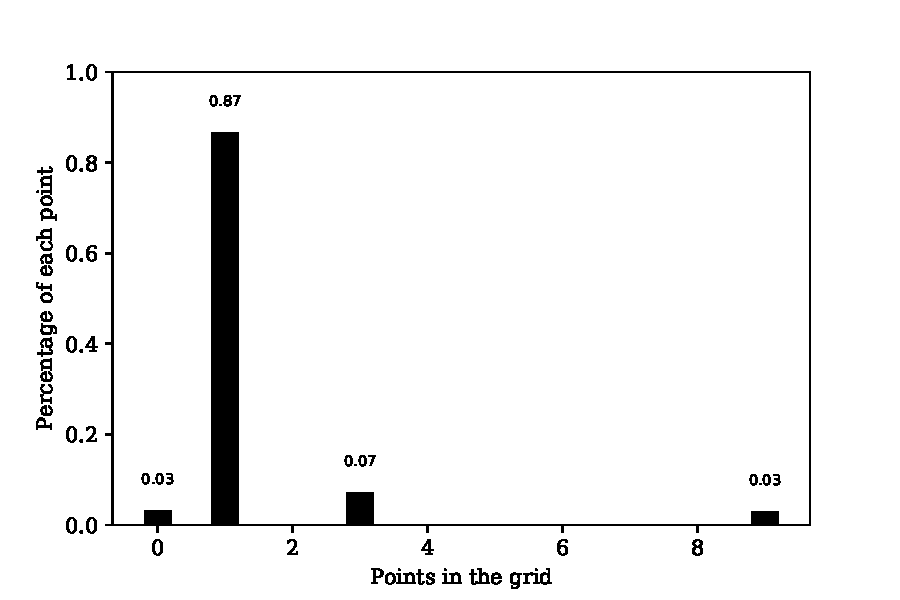
\includegraphics[width=0.9\textwidth]{average_percentagenorm1_200_3000_500}
		\caption{percentage of converging to the best, average of 500 time run, Histogram}\label{average_percentagenorm1_200_3000_500}
	\end{figure}
	\begin{figure}[H]
		\centering
		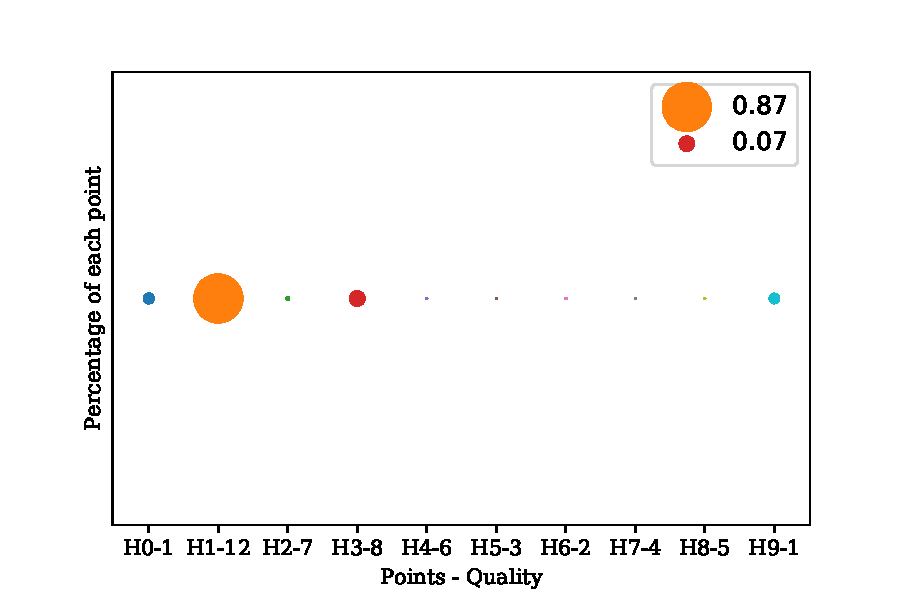
\includegraphics[width=0.9\textwidth]{Average_percentagenorm1_200_3000_500_2}
		\caption{average percentage average of choosing to the best, average of 500 time run, circle}\label{Average_percentagenorm1_200_3000_500_2}
	\end{figure}
	\begin{figure}[H]
		\centering
		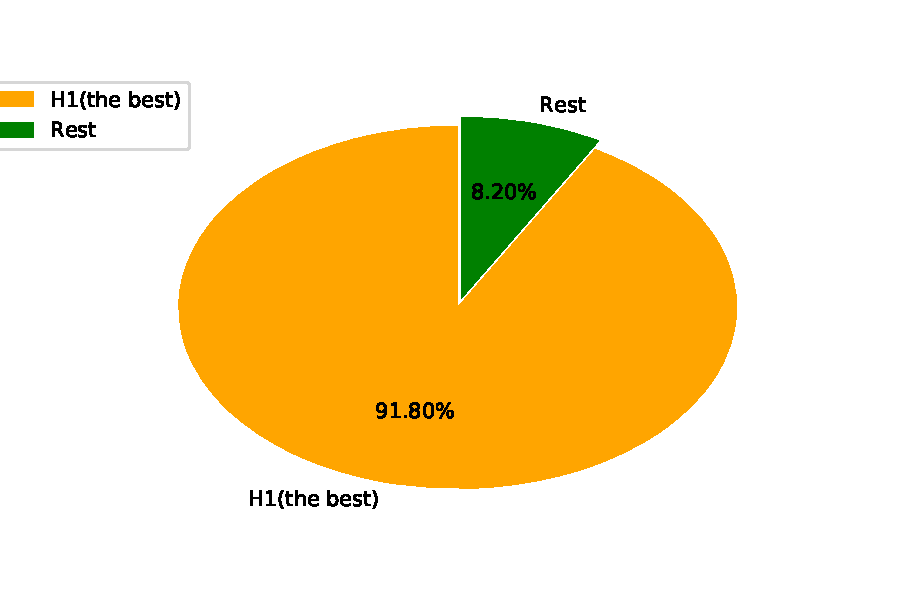
\includegraphics[width=0.9\textwidth]{average_percentagenorm1_200_3000_500_3}
		\caption{percentage of converging to the best, average of 500 time run, pie}\label{average_percentagenorm1_200_3000_500_3}
	\end{figure}
	
	\begin{figure}[H]
		\centering
		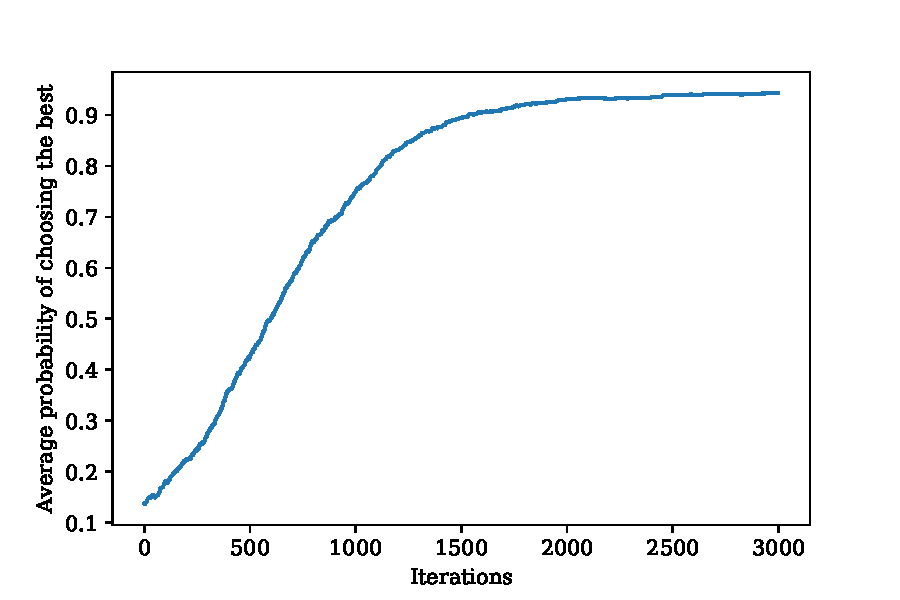
\includegraphics[width=0.9\textwidth]{correct_pbestnorm1_200_3000_500}
		\caption{Probability for choosing the best against iteration time, average of 500 time run, only when converge to the best of n(H1)}\label{correct_pbestnorm1_200_3000_500}
	\end{figure}
	\begin{figure}[H]
		\centering
		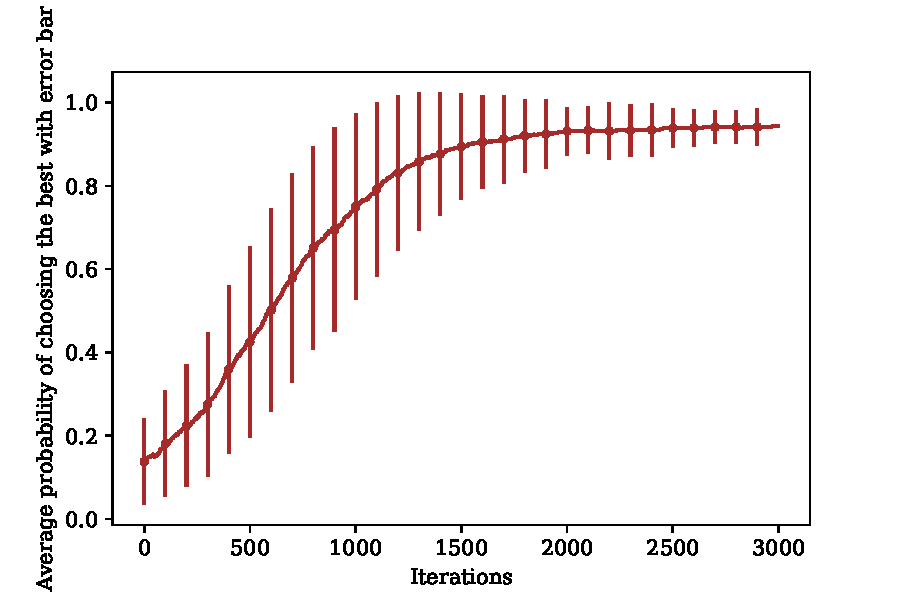
\includegraphics[width=0.9\textwidth]{correct_pbest_errbarnorm1_200_3000_500}
		\caption{Probability for choosing the best against iteration time, average of 500 time run, only when converge to the best of n(H1), with error bar}\label{correct_pbest_errbarnorm1_200_3000_500}
	\end{figure}
	%
	\begin{figure}[H]
		\centering
		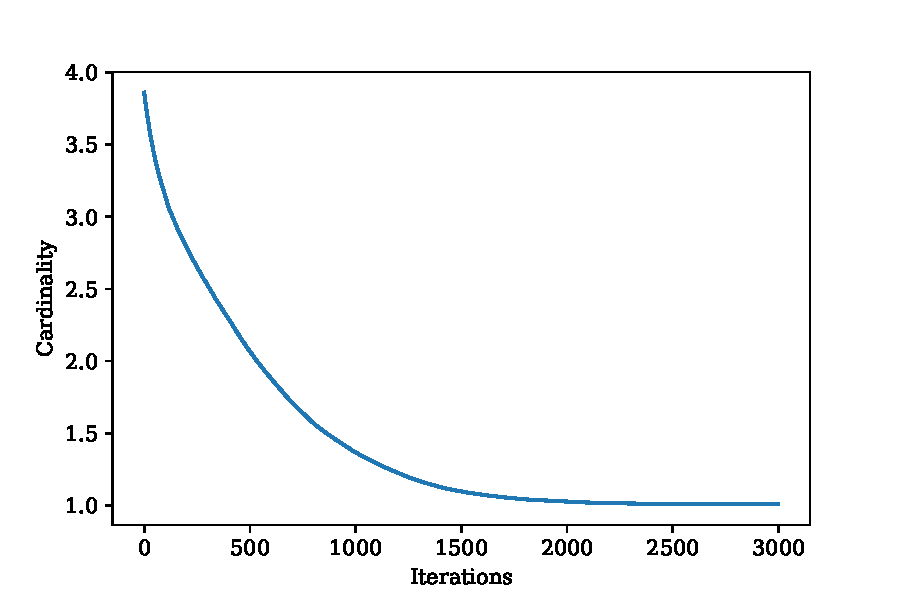
\includegraphics[width=0.9\textwidth]{cardnorm1_200_3000_500}
		\caption{Cardinality against iteration time, average of 500 time run}\label{cardnorm1_200_3000_500}
	\end{figure}
	\begin{figure}[H]
		\centering
		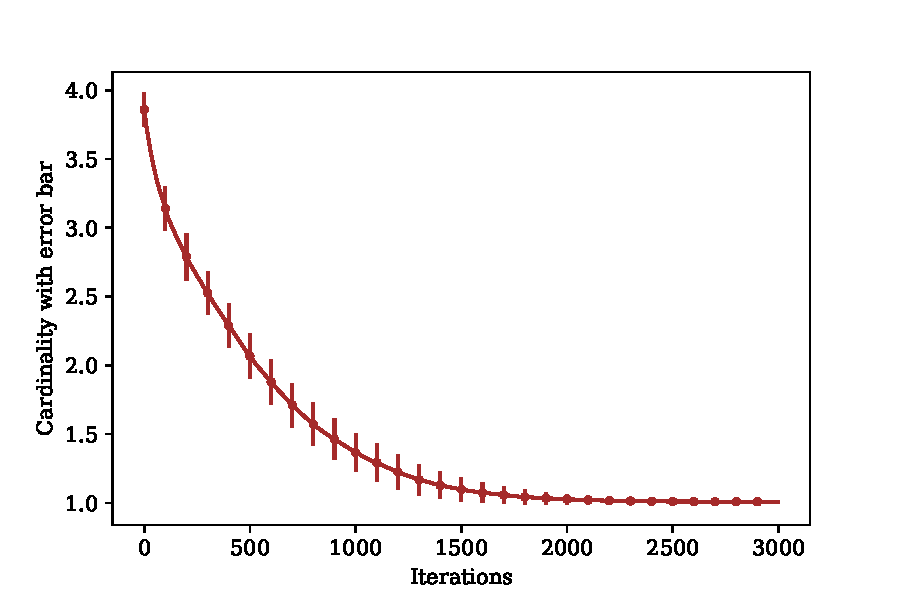
\includegraphics[width=0.9\textwidth]{card_errbarnorm1_200_3000_500}
		\caption{Cardinality against iteration time, average of 500 time run, with error bar}\label{card_errbarnorm1_200_3000_500}
	\end{figure}
\subsection{Toss coin initialising,	100 times experiments}\label{tcsqrank}

	Grid : Q = \{'H0':1,'H1': 12, 'H2': 7, 'H3': 8, 'H4': 6,'H5': 3,'H6': 2,'H7': 4,'H8':5,'H9':1\}
	The probability was determined by the square of rank of points' qualities.
	\graphicspath{{figsNorm1/}}
	Time used: forget to record%~${s}$
	\begin{figure}[H]
		\centering
		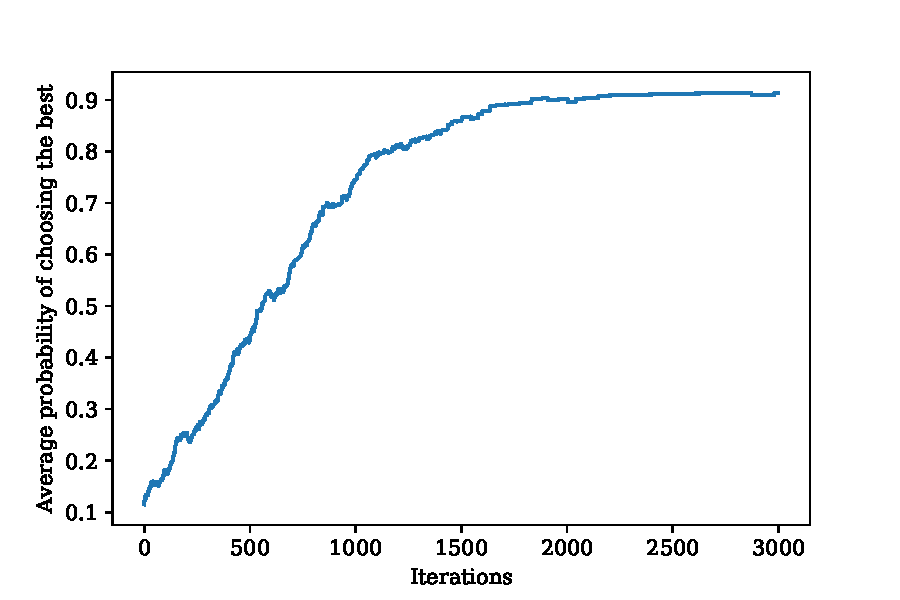
\includegraphics[width=0.9\textwidth]{Average_pbestnorm1_toss200_3000_100}
		\caption{Probability for choosing the best against iteration time, average of 100 time run}\label{Average_pbestnorm1_toss200_3000_100}
	\end{figure}
	%
	\begin{figure}[H]
		\centering
		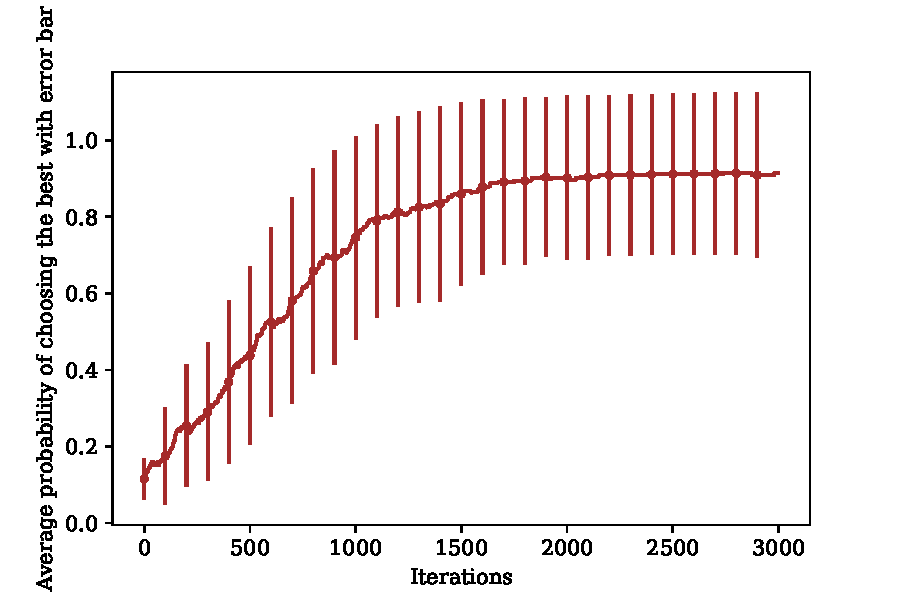
\includegraphics[width=0.9\textwidth]{Average_pbest_errbarnorm1_toss200_3000_100}
		\caption{Probability for choosing the best against iteration time, average of 100 time run, with error bar}\label{Average_pbest_errbarnorm1_toss200_3000_100}
	\end{figure}
	%
	\begin{figure}[H]
		\centering
		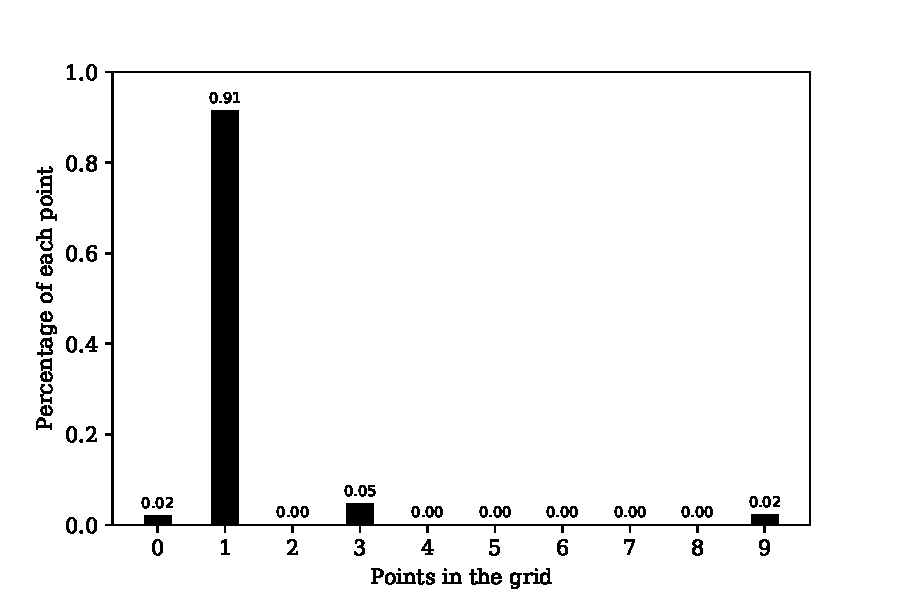
\includegraphics[width=0.9\textwidth]{average_percentagenorm1_toss200_3000_100}
		\caption{percentage of converging to the best, average of 100 time run, Histogram}\label{average_percentagenorm1_toss200_3000_100}
	\end{figure}
	\begin{figure}[H]
		\centering
		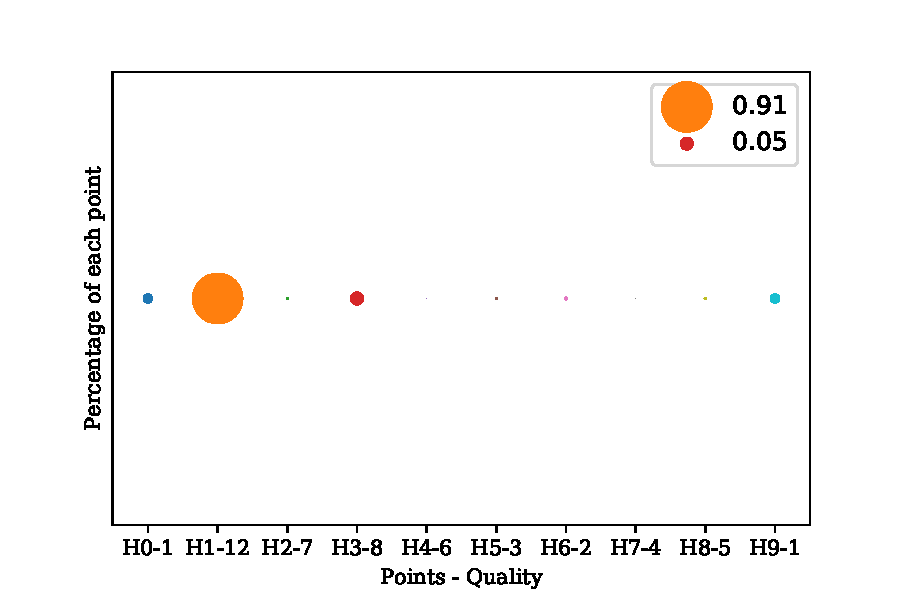
\includegraphics[width=0.9\textwidth]{Average_percentagenorm1_toss200_3000_100_2}
		\caption{average percentage average of choosing to the best, average of 100 time run, circle}\label{Average_percentagenorm1_toss200_3000_100_2}
	\end{figure}
	\begin{figure}[H]
		\centering
		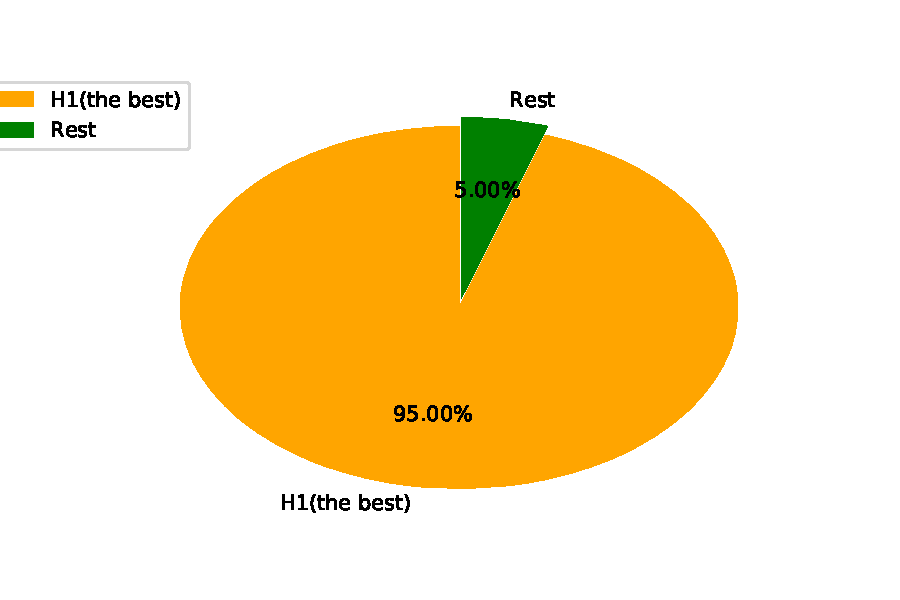
\includegraphics[width=0.9\textwidth]{average_percentagenorm1_toss200_3000_100_3}
		\caption{percentage of converging to the best, average of 100 time run, pie}\label{average_percentagenorm1_toss200_3000_100_3}
	\end{figure}
	
	\begin{figure}[H]
		\centering
		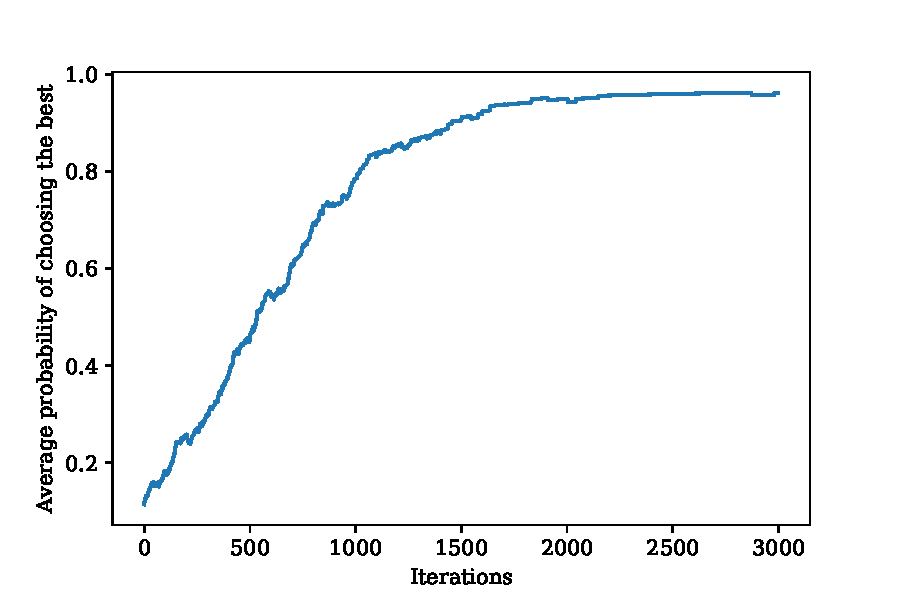
\includegraphics[width=0.9\textwidth]{correct_pbestnorm1_toss200_3000_100}
		\caption{Probability for choosing the best against iteration time, average of 100 time run, only when converge to the best of n(H1)}\label{correct_pbestnorm1_toss200_3000_100}
	\end{figure}
	\begin{figure}[H]
		\centering
		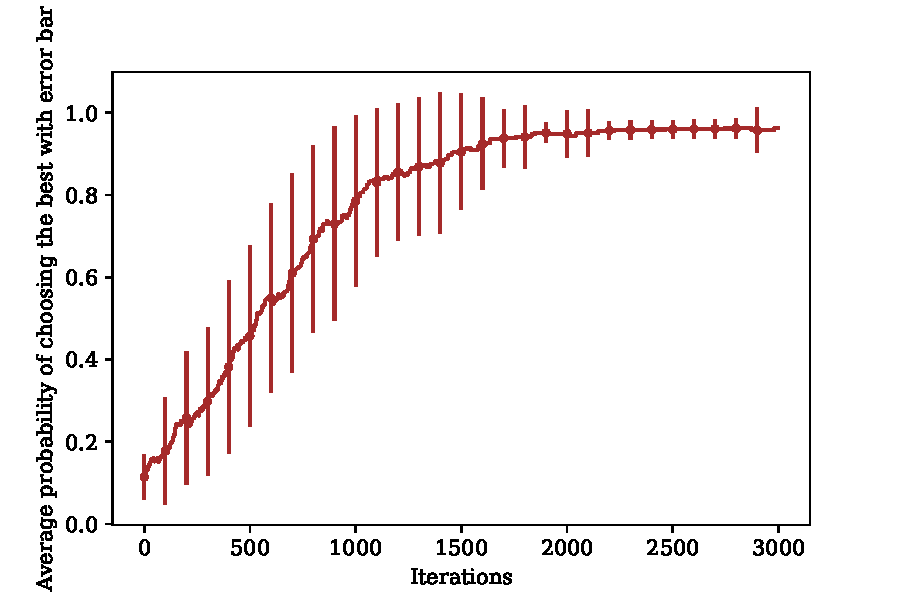
\includegraphics[width=0.9\textwidth]{correct_pbest_errbarnorm1_toss200_3000_100}
		\caption{Probability for choosing the best against iteration time, average of 100 time run, only when converge to the best of n(H1), with error bar}\label{correct_pbest_errbarnorm1_toss200_3000_100}
	\end{figure}
	%
	\begin{figure}[H]
		\centering
		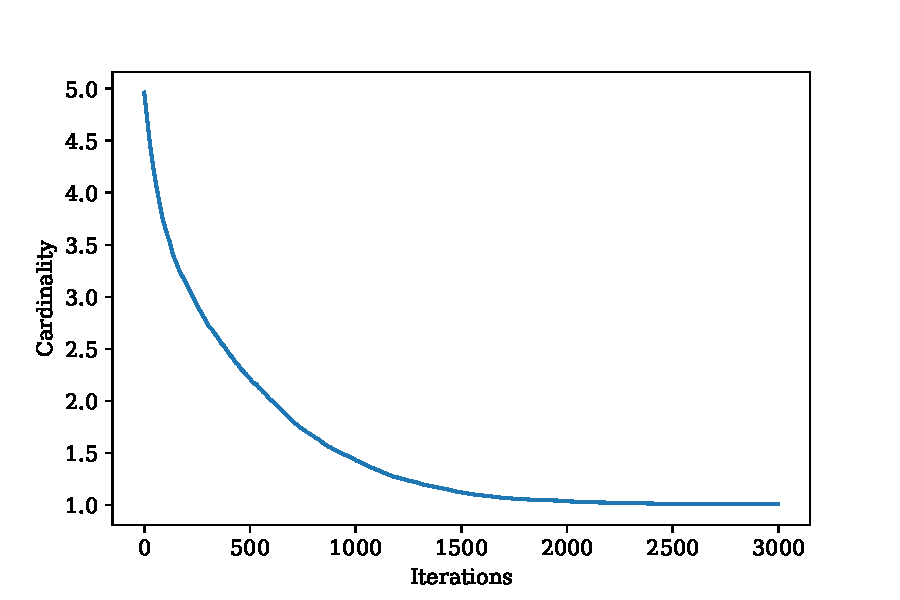
\includegraphics[width=0.9\textwidth]{cardnorm1_toss200_3000_100}
		\caption{Cardinality against iteration time, average of 100 time run}\label{cardnorm1_toss200_3000_100}
	\end{figure}
	\begin{figure}[H]
		\centering
		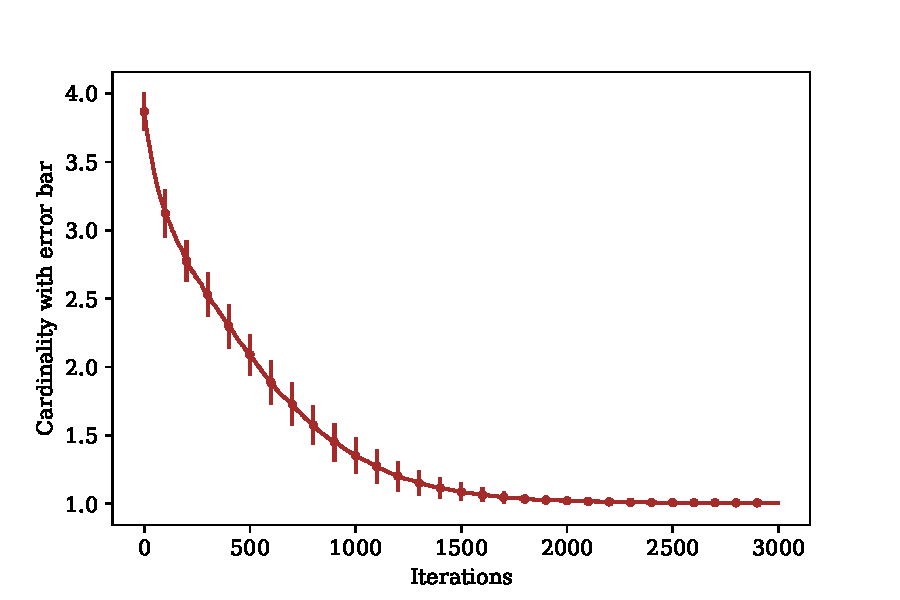
\includegraphics[width=0.9\textwidth]{card_errbarnorm1_200_3000_100}
		\caption{Cardinality against iteration time, average of 100 time run, with error bar}\label{card_errbarnorm1_toss200_3000_100}
	\end{figure}
\end{document}
